\chapter{Tools and technologies}
\label{chapter5}

In this chapter, we will thoroughly describe the tools, technologies and other materials that were utilized in any way to help in the development of this Degree Final Project. This includes any necessary programming languages, plugins, IDEs, APIs, database engines, data sources and any other software development and documentation tools that were needed at any stage of the process for building the mobile application.

Besides, for some of them we will also provide a comparison with other similar options and justify why it was finally decided to choose them for this project over the rest of available solutions. The tools and technologies that were used to plan and develop the mobile application are the following:

\section{Version control}

In this section we will briefly describe the tools used to maintain a version control of the project source files and documentation.

\subsection{Git}

For efficiently keeping track of any changes made in the project code and documentation files we utilized Git \cite{noauthor_git_2021}. Git is a free and open-source version control software whose main purpose is registering any changes made on the project files, allowing to coordinate and synchronize the work across members of a team that are working on the same code. Git's logotype is shown in Figure \ref{fig:git}.

\begin{figure}[h]
  \centering
  
\includegraphics[width=0.5\textwidth]{Figures/git-logo.png}
  \caption{%
    Git's logotype
  }
  \label{fig:git}
\end{figure}

Even though the team is solely composed of one member, Git has been used to rollback to previous versions whenever needed, as well as to easily share any modifications with the project's director. It was also chosen because of the multiple integrations available with other tools such as Visual Studio Code or Overleaf. 

Git is also a distributed system, which means that the complete codebase (the files generated by the version control) is stored on the user computer instead of only on the server like in centralized client-server systems like such as Subversion \cite{noauthor_apache_nodate} or CVS \cite{noauthor_cvs_nodate}. Figure \ref{fig:git-repo} shows the repository structure and the files generated by Git in Git Bash, a CLI tool provided by the default installation.

\begin{figure}[h]
  \centering
  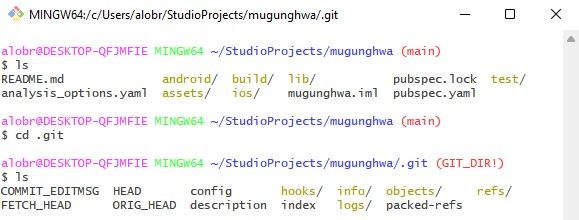
\includegraphics[width=0.75\textwidth]{Figures/git-repo.png}
  \caption{%
    Repository and files generated by Git
  }
  \label{fig:git-repo}
\end{figure}

Despite being a decentralized system, we also made use of a centralized platform for hosting our Git repository while having access to several additional features such as issue tracking, Kanban boards, \textit{wikis}, etc. This centralized hosting service is GitHub.

\subsection{GitHub}

GitHub \cite{noauthor_githubcom_2021} is a platform dedicated to provide hosting and version control services using Git for the source code of any software project. The projects stored in GitHub servers are typically public and available for everyone, as it is mainly a platform dedicated for open-source and collaborative projects. However, it also offers the possibility to open private repositories, first as a paid feature but available for free users too since April 2020. 

\begin{figure}[h]
  \centering
  
\includegraphics[width=0.5\textwidth]{Figures/github-logo.png}
  \caption{%
    GitHub's logotype
  }
  \label{fig:github-logo}
\end{figure}

[link al/los repos]

\section{Documentation}

\subsection{\LaTeX}

\subsection{Overleaf}

\subsection{Zotero}

\subsection{Microsoft Project}

\begin{itemize}
\item During the preprocessing of the input images, use will be made of the OpenCV \cite{noauthor_opencv_2021} library for artificial vision, open source and available for Python \cite{noauthor_python_2021} through OpenCV-Python \cite{noauthor_opencv-python_2021}.
\item To capture the text, we will work with the Tesseract \cite{noauthor_tesseract_2021} optical character recognition engine, also open source, and with the Python-tesseract wrapper \cite{lee_pytesseract_2021}.
\item In the case of post-processing the text and obtaining the list of ingredients, use will be made of the library of tools for natural language processing NLTK \cite{noauthor_natural_2021}.
\item The database will be created and maintained using the MySQL relational management system \cite{noauthor_mysql_2021}.
\item The application for Android devices will be implemented using the Flutter software development kit \cite{noauthor_flutter_2021}.
\item The development of all the code will be done using the Visual Studio Code text editor \cite{noauthor_documentation_2021}, as well as the Android Studio IDE \cite{noauthor_introduccion_2021}. The source code control will be done with Git \cite{noauthor_git_2021} and GitHub \cite{noauthor_githubcom_2021}.
\end{itemize}